% ============================================================================
% Integración SUMO-GEO (visor 3D web) + VaN3Twin (ns-3) vía TraCI multi-cliente
% Universidad de Cuenca — Redes Vehiculares y Heterogéneas (INGE-00104)
% Compilar: pdflatex -interaction=nonstopmode Integracion_SUMO_GEO_VaN3Twin.tex (x2)
% ============================================================================
\documentclass[11pt,a4paper]{article}

\usepackage[utf8]{inputenc}
\usepackage[T1]{fontenc}
\usepackage{lmodern}
\usepackage[margin=2.2cm]{geometry}
\usepackage{xcolor}
\usepackage{graphicx}
\usepackage{booktabs}
\usepackage{enumitem}
\usepackage{fancyhdr}
\usepackage{tikz}
\usetikzlibrary{positioning,arrows.meta,shapes.geometric,calc}
\usepackage{listings}
\usepackage[most]{tcolorbox}
\usepackage{hyperref}

% ----------------------------------------------------------------------------
% Colores institucionales
% ----------------------------------------------------------------------------
\definecolor{azul}{HTML}{002856}
\definecolor{rojo}{HTML}{A51008}
\definecolor{gris}{HTML}{58585B}
\definecolor{verde}{HTML}{1A7A4A}
\definecolor{fondocodigo}{HTML}{F5F5F5}

\hypersetup{colorlinks=true, linkcolor=azul, urlcolor=rojo, citecolor=azul}

\pagestyle{fancy}
\fancyhf{}
\fancyhead[L]{\small\color{azul}\textbf{SUMO-GEO + VaN3Twin}}
\fancyhead[R]{\small\color{gris}Redes Vehiculares y Heterogéneas}
\fancyfoot[C]{\small\thepage}
\renewcommand{\headrulewidth}{0.6pt}

% ----------------------------------------------------------------------------
% Listados de código
% ----------------------------------------------------------------------------
\lstdefinestyle{codigo}{
  backgroundcolor=\color{fondocodigo},
  basicstyle=\ttfamily\footnotesize,
  keywordstyle=\color{azul}\bfseries,
  commentstyle=\color{verde}\itshape,
  stringstyle=\color{rojo},
  numbers=none,
  breaklines=true,
  frame=single,
  rulecolor=\color{gris!40},
  framesep=4pt,
  showstringspaces=false,
  tabsize=2,
  columns=fullflexible,
  keepspaces=true
}
\lstset{style=codigo}

% ----------------------------------------------------------------------------
% Cajas "dónde se ejecuta cada paso"
% ----------------------------------------------------------------------------
\newtcolorbox{enmac}[1][]{
  colback=azul!4, colframe=azul, fonttitle=\bfseries, breakable,
  title={\faIconMac~EN EL MAC (PC local) #1}}
\newtcolorbox{encontenedor}[1][]{
  colback=rojo!4, colframe=rojo, fonttitle=\bfseries, breakable,
  title={\faIconDocker~DENTRO DEL CONTENEDOR \texttt{van3twin} #1}}
\newtcolorbox{enrepo}[1][]{
  colback=verde!5, colframe=verde, fonttitle=\bfseries, breakable,
  title={\faIconEdit~EN EL MAC — editar archivos del repo \texttt{SUMO\_GEO} #1}}
\newtcolorbox{notabox}[1][]{
  colback=gris!6, colframe=gris, fonttitle=\bfseries, breakable,
  title={Nota#1}}
\newtcolorbox{validadobox}{
  colback=verde!6, colframe=verde, fonttitle=\bfseries, breakable,
  title={Validado empíricamente}}
\newtcolorbox{tallerbox}{
  colback=azul!5, colframe=azul, fonttitle=\bfseries, breakable,
  title={TAREA DEL TALLER}}

% "iconos" simples (sin fuentes extra)
\newcommand{\faIconMac}{\tikz[baseline=-2pt]{\draw[azul,fill=azul!15,rounded corners=1pt] (0,0) rectangle (0.32,0.22); \draw[azul] (0.10,-0.05)--(0.22,-0.05);}}
\newcommand{\faIconDocker}{\tikz[baseline=-2pt]{\foreach \x in {0,0.11,0.22}{\draw[rojo,fill=rojo!15] (\x,0) rectangle (\x+0.09,0.09);}\foreach \x in {0.055,0.165}{\draw[rojo,fill=rojo!15] (\x,0.11) rectangle (\x+0.09,0.2);}}}
\newcommand{\faIconEdit}{\tikz[baseline=-2pt]{\draw[verde,fill=verde!15] (0,0) -- (0.22,0.22) -- (0.28,0.16) -- (0.06,-0.06) -- cycle;}}

\setlength{\parskip}{4pt}
\setlength{\parindent}{0pt}

% ============================================================================
\begin{document}

\begin{center}
  {\color{azul}\LARGE\bfseries Integración SUMO-GEO + VaN3Twin}\\[4pt]
  {\color{gris}\large Visor web 3D (MapLibre/deck.gl) conectado en vivo a la simulación V2X de ns-3}\\[6pt]
  {\small Universidad de Cuenca --- Redes Vehiculares y Heterogéneas (INGE-00104)\\
  Prof.\ Pablo Barbecho --- \today}
\end{center}

\vspace{2pt}
\hrule
\vspace{8pt}

\tableofcontents

% ============================================================================
\section{Objetivo y mecanismo}
% ============================================================================

\textbf{Objetivo:} que la plataforma \href{https://github.com/Pbarbecho/SUMO_GEO}{SUMO-GEO}
(FastAPI + MapLibre GL~JS + deck.gl, desplegada con Docker) visualice en 3D y en tiempo
real \emph{la misma simulación SUMO que controla VaN3Twin} (ns-3), en lugar de lanzar su
propio SUMO.

\textbf{Mecanismo:} TraCI \textbf{multi-cliente}. SUMO admite varios clientes TraCI
simultáneos si se arranca con \texttt{--num-clients~N}; cada cliente declara su turno con
\texttt{setOrder(k)} y la simulación avanza en \emph{lockstep}: SUMO solo ejecuta un paso
cuando \emph{todos} los clientes lo han solicitado.

\begin{itemize}[leftmargin=1.4em]
  \item \textbf{Cliente 1} $\rightarrow$ VaN3Twin (ns-3): controla la movilidad, inyecta
        los vehículos, ejecuta la pila ITS-G5 (CAM/DENM) y las métricas.
  \item \textbf{Cliente 2} $\rightarrow$ backend de SUMO-GEO en modo \texttt{remote}:
        \emph{solo lee} (suscripciones de posición, velocidad, CO$_2$, semáforos) y
        alimenta el visor 3D del navegador.
\end{itemize}

SUMO-GEO ya incluye el modo \texttt{APP\_SUMO\_MODE=remote} para conectarse a un SUMO
externo; la integración requiere únicamente \textbf{dos parches pequeños} (uno por lado)
más el cableado Docker (red compartida y carpeta local montada).

% ============================================================================
\section{Arquitectura resultante}
% ============================================================================

\begin{figure}[h]
\centering
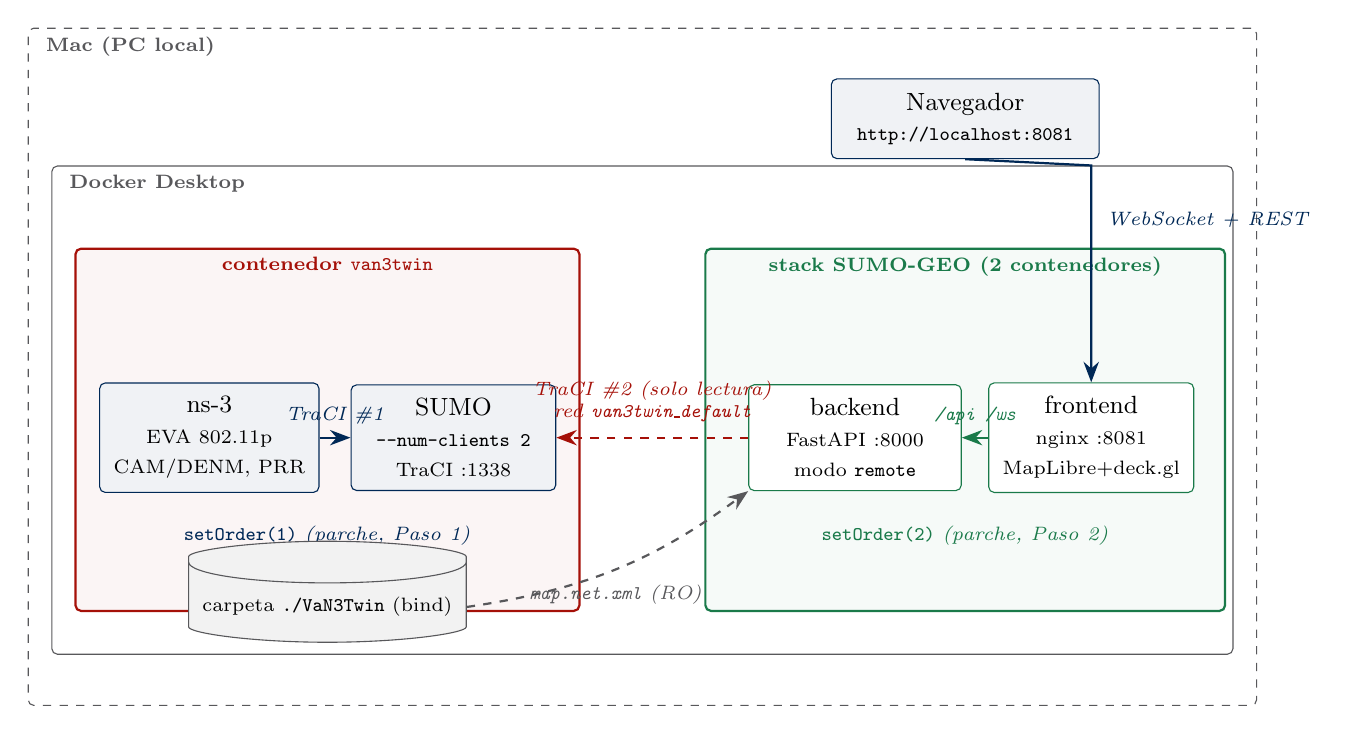
\begin{tikzpicture}[
  font=\small,
  caja/.style={draw, rounded corners=2pt, align=center, inner sep=5pt},
  flecha/.style={-{Stealth[length=2.6mm]}, thick},
  etiq/.style={font=\scriptsize\itshape, midway}
]
  % --- Mac (marco exterior)
  \node[caja, draw=gris, dashed, minimum width=15.6cm, minimum height=8.6cm] (mac) at (0,0) {};
  \node[anchor=north west, font=\scriptsize\bfseries\color{gris}] at (mac.north west) {~Mac (PC local)};

  % --- Docker Desktop (marco interior)
  \node[caja, draw=gris, minimum width=15cm, minimum height=6.2cm] (docker) at (0,-0.55) {};
  \node[anchor=north west, font=\scriptsize\bfseries\color{gris}] at (docker.north west) {~Docker Desktop};

  % --- contenedor van3twin
  \node[caja, draw=rojo, thick, fill=rojo!4, minimum width=6.4cm, minimum height=4.6cm]
        (van) at (-4,-0.8) {};
  \node[anchor=north, font=\scriptsize\bfseries\color{rojo}] at (van.north) {contenedor \texttt{van3twin}};
  \node[caja, draw=azul, fill=azul!6, minimum width=2.6cm] (ns3) at (-5.5,-0.9)
        {ns-3\\\scriptsize EVA 802.11p\\\scriptsize CAM/DENM, PRR};
  \node[caja, draw=azul, fill=azul!6, minimum width=2.6cm] (sumo) at (-2.4,-0.9)
        {SUMO\\\scriptsize \texttt{--num-clients 2}\\\scriptsize TraCI :1338};
  \draw[flecha, azul] (ns3) -- (sumo) node[etiq, above=1pt] {TraCI \#1};
  \node[font=\scriptsize\color{azul}] at (-4,-2.15) {\texttt{setOrder(1)} \emph{(parche, Paso 1)}};
  % volumen
  \node[caja, draw=gris, fill=gris!8, cylinder, shape border rotate=90, aspect=0.15,
        minimum width=2.9cm, minimum height=0.85cm, font=\scriptsize]
        (vol) at (-4,-3.05) {carpeta \texttt{./VaN3Twin} (bind)};

  % --- stack SUMO-GEO
  \node[caja, draw=verde, thick, fill=verde!4, minimum width=6.6cm, minimum height=4.6cm]
        (geo) at (4.1,-0.8) {};
  \node[anchor=north, font=\scriptsize\bfseries\color{verde}] at (geo.north) {stack SUMO-GEO (2 contenedores)};
  \node[caja, draw=verde, fill=white, minimum width=2.7cm] (backend) at (2.7,-0.9)
        {backend\\\scriptsize FastAPI :8000\\\scriptsize modo \texttt{remote}};
  \node[caja, draw=verde, fill=white, minimum width=2.6cm] (nginx) at (5.7,-0.9)
        {frontend\\\scriptsize nginx :8081\\\scriptsize MapLibre+deck.gl};
  \node[font=\scriptsize\color{verde}] at (4.1,-2.15) {\texttt{setOrder(2)} \emph{(parche, Paso 2)}};
  \draw[flecha, verde] (nginx) -- (backend) node[etiq, above=1pt] {\texttt{/api /ws}};

  % --- red docker compartida
  \draw[flecha, rojo, dashed, thick] (backend.west) -- (sumo.east)
        node[etiq, above=2pt, align=center] {TraCI \#2 (solo lectura)\\red \texttt{van3twin\_default}};
  % volumen -> backend (net.xml)
  \draw[flecha, gris, dashed] (vol.east) to[bend right=14]
        node[etiq, below=2pt] {\texttt{map.net.xml} (RO)} (backend.south west);

  % --- navegador
  \node[caja, draw=azul, fill=azul!6, minimum width=3.4cm] (browser) at (4.1,3.15)
        {Navegador\\\scriptsize \texttt{http://localhost:8081}};
  \draw[flecha, azul, thick] (browser.south) -- (nginx.north |- docker.north) -- (nginx.north)
        node[etiq, right=2pt, pos=0.25] {WebSocket + REST};
\end{tikzpicture}
\caption{Arquitectura: dos proyectos Docker Compose independientes unidos por la red
\texttt{van3twin\_default} (TraCI) y la carpeta local \texttt{VaN3Twin} del Mac (bind mount, geometría del mapa).}
\label{fig:arq}
\end{figure}

\begin{validadobox}
Antes de escribir esta guía se validó la mecánica en un entorno de pruebas
(SUMO~1.27 + \texttt{traci}), con estos resultados:
\begin{enumerate}[leftmargin=1.6em, itemsep=1pt]
  \item \textbf{Lockstep sin bloqueo mutuo}: cliente~1 con pasos finos (0{,}1~s) +
        cliente~2 pidiendo objetivos gruesos (\texttt{simulationStep(t+1.0)})
        $\Rightarrow$ el visor \emph{no} frena a ns-3.
  \item \textbf{El handshake del cliente~1 queda bloqueado} hasta que conecta el
        cliente~2: tras lanzar la simulación, ns-3 ``espera'' hasta abrir el visor.
  \item \texttt{setOrder(1)} es \textbf{inocuo con un solo cliente}: el parche de
        VaN3Twin no altera el uso normal.
  \item SUMO escucha TraCI en \texttt{0.0.0.0} $\Rightarrow$ es alcanzable desde otro
        contenedor por la red Docker \textbf{sin publicar el puerto} al Mac.
\end{enumerate}
\end{validadobox}

% ============================================================================
\section{Mapa de la guía: qué se hace y dónde}
% ============================================================================

Cada paso indica su ubicación con una caja de color:
\textcolor{rojo}{\textbf{rojo}} = dentro del contenedor \texttt{van3twin};
\textcolor{verde}{\textbf{verde}} = editar archivos del repo \texttt{SUMO\_GEO} en el Mac;
\textcolor{azul}{\textbf{azul}} = terminal del Mac (PC local).

\begin{figure}[h]
\centering
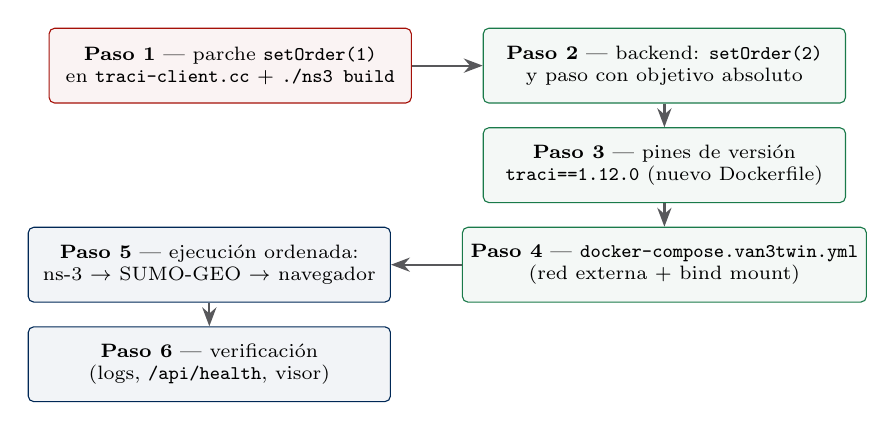
\begin{tikzpicture}[
  font=\scriptsize, node distance=3mm,
  paso/.style={draw, rounded corners=2pt, align=center, minimum width=4.6cm,
               minimum height=0.95cm, inner sep=3pt},
  flecha/.style={-{Stealth[length=2.4mm]}, thick, gris}
]
  \node[paso, draw=rojo, fill=rojo!5]  (p1) {\textbf{Paso 1} — parche \texttt{setOrder(1)}\\en \texttt{traci-client.cc} + \texttt{./ns3 build}};
  \node[paso, draw=verde, fill=verde!5, right=9mm of p1] (p2) {\textbf{Paso 2} — backend: \texttt{setOrder(2)}\\y paso con objetivo absoluto};
  \node[paso, draw=verde, fill=verde!5, below=of p2] (p3) {\textbf{Paso 3} — pines de versión\\\texttt{traci==1.12.0} (nuevo Dockerfile)};
  \node[paso, draw=verde, fill=verde!5, below=of p3] (p4) {\textbf{Paso 4} — \texttt{docker-compose.van3twin.yml}\\(red externa + bind mount)};
  \node[paso, draw=azul, fill=azul!5, left=9mm of p4]  (p5) {\textbf{Paso 5} — ejecución ordenada:\\ns-3 $\rightarrow$ SUMO-GEO $\rightarrow$ navegador};
  \node[paso, draw=azul, fill=azul!5, below=of p5] (p6) {\textbf{Paso 6} — verificación\\(logs, \texttt{/api/health}, visor)};
  \draw[flecha] (p1) -- (p2);
  \draw[flecha] (p2) -- (p3);
  \draw[flecha] (p3) -- (p4);
  \draw[flecha] (p4) -- (p5);
  \draw[flecha] (p5) -- (p6);
\end{tikzpicture}
\caption{Secuencia de pasos y ubicación de cada uno (color).}
\end{figure}

\begin{notabox}[: requisitos previos (Paso 0)]
\begin{itemize}[leftmargin=1.4em, itemsep=1pt]
  \item Stack \texttt{van3twin-docker} construido y funcional (imagen \texttt{van3twin:jammy}).
  \item Repo \texttt{SUMO\_GEO} clonado en el Mac:
        \texttt{git clone https://github.com/Pbarbecho/SUMO\_GEO}.
  \item Puertos libres en el Mac: \texttt{8081} (frontend) y \texttt{8000} (backend).
        El puerto TraCI \texttt{1338} \emph{no} se publica: viaja solo por la red interna de Docker.
\end{itemize}
\end{notabox}

% ============================================================================
\section{Paso 1 — Parche en VaN3Twin: \texttt{setOrder(1)}}
% ============================================================================

El cliente TraCI de VaN3Twin (\texttt{src/traci/model/traci-client.cc}) \emph{nunca} llama a
\texttt{setOrder()}, aunque su API lo implementa (\texttt{sumo-TraCIAPI.cc:87}). Sin esa
llamada, SUMO multi-cliente no conoce el turno del cliente y la simulación se bloquea.
El parche añade la llamada justo después de \texttt{TraCIAPI::connect()} (línea $\approx$282),
\textbf{condicionada} a que se haya pedido \texttt{--num-clients}: el uso normal de
VaN3Twin no cambia en absoluto.

\begin{encontenedor}[ --- editar y recompilar (persiste en \texttt{./VaN3Twin} del Mac)]
\begin{lstlisting}[language=bash]
# en el Mac: entrar al contenedor
cd ~/van3twin-docker && docker compose up -d
docker compose exec van3twin bash

# dentro del contenedor:
cd ~/VaN3Twin/ns-3-dev
sed -i '/this->TraCIAPI::connect("localhost", m_sumoPort);/a\
        if (m_sumoAddCmdOpt.find("--num-clients") != std::string::npos) { this->TraCIAPI::setOrder(1); }' \
  src/traci/model/traci-client.cc

./ns3 build     # recompila solo el modulo traci y sus dependientes
\end{lstlisting}
El resultado, en contexto, queda así:
\begin{lstlisting}[language=C++]
// connect to sumo via traci
try
  {
    this->TraCIAPI::connect("localhost", m_sumoPort);
    if (m_sumoAddCmdOpt.find("--num-clients") != std::string::npos)
      { this->TraCIAPI::setOrder(1); }   // <-- NUEVO (parche)
  }
catch (std::exception& e) { ... }
\end{lstlisting}
\end{encontenedor}

\begin{notabox}[: hacer el parche permanente (opcional)]
El cambio anterior vive en la carpeta local \texttt{van3twin-docker/VaN3Twin} del Mac
(bind mount), así que persiste siempre, incluso si se elimina el contenedor. Para
hornearlo además en la imagen, añade el mismo \texttt{sed} como capa \texttt{RUN} en el \texttt{Dockerfile} de
\texttt{van3twin-docker} (antes de la capa de \texttt{configure/build}) y reconstruye.
\end{notabox}

% ============================================================================
\section{Paso 2 — Parche en SUMO-GEO: \texttt{setOrder(2)} y paso absoluto}
% ============================================================================

Dos archivos del backend. Primero, un nuevo parámetro de configuración:

\begin{enrepo}[ --- \texttt{backend/app/config.py}]
Añadir tras \texttt{sumo\_port}:
\begin{lstlisting}[language=Python]
    sumo_order: int = 0   # >0 => TraCI multi-cliente: llamar setOrder(N) al conectar
\end{lstlisting}
(Se controla con la variable de entorno \texttt{APP\_SUMO\_ORDER}; con el valor por
defecto \texttt{0} el comportamiento actual no cambia.)
\end{enrepo}

\begin{enrepo}[ --- \texttt{backend/app/sumo\_bridge.py} (2 cambios)]
\textbf{(a)} En \texttt{start()}, rama \texttt{remote}:
\begin{lstlisting}[language=Python]
        if settings.sumo_mode == "remote" and not self._libsumo:
            client.init(host=settings.sumo_host, port=settings.sumo_port)
            if settings.sumo_order:
                client.setOrder(settings.sumo_order)     # <-- NUEVO
            self.conn = client
\end{lstlisting}
\textbf{(b)} En \texttt{step()} --- el cambio \emph{crítico}:
\begin{lstlisting}[language=Python]
    def step(self) -> float:
        if settings.sumo_mode == "remote" and settings.sumo_order:
            # objetivo ABSOLUTO grueso: ns-3 marca el ritmo con sus pasos finos
            self.conn.simulationStep(
                self.conn.simulation.getTime() + settings.step_length)
        else:
            self.conn.simulationStep()
        # ... resto del metodo sin cambios ...
\end{lstlisting}
\end{enrepo}

\subsection*{Por qué el objetivo absoluto es imprescindible}

VaN3Twin lanza SUMO con \texttt{--step-length} igual a su intervalo de sincronización
(pasos finos, p.\,ej.\ 0{,}01--0{,}1~s). En la barrera multi-cliente, si el visor pidiera
``un paso'' por frame (10~fps), ns-3 quedaría esclavo del visor: $10$ pasos de $0{,}1$~s
por segundo real $=$ simulación $10\times$ más lenta. Con el objetivo absoluto
\texttt{t+1.0}, el visor concede un margen amplio y ns-3 avanza a su propio ritmo
(hecho validado \#1).

\begin{figure}[h]
\centering
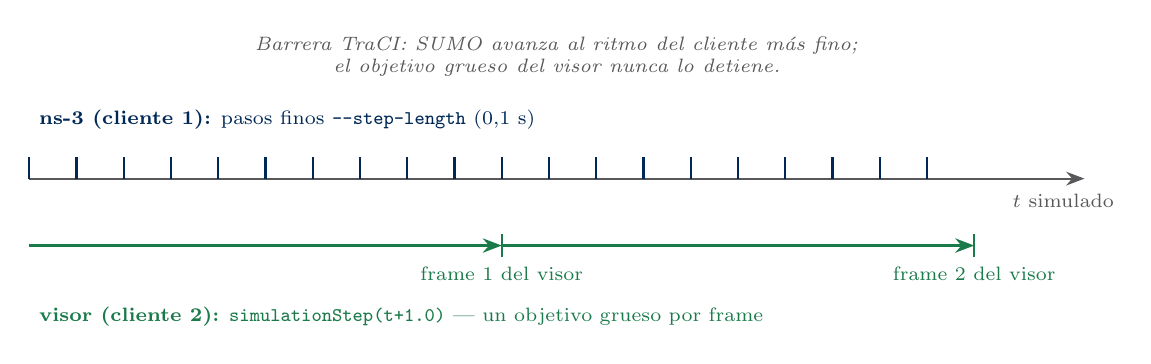
\begin{tikzpicture}[font=\scriptsize]
  % eje de tiempo simulado
  \draw[-{Stealth}, thick, gris] (0,0) -- (13.4,0) node[below=2pt, pos=0.98] {$t$ simulado};
  % pasos finos ns-3
  \foreach \x in {0,0.6,...,12}{\draw[azul, thick] (\x,0) -- (\x,0.28);}
  \node[azul, anchor=west] at (0,0.75) {\textbf{ns-3 (cliente 1):} pasos finos \texttt{--step-length} (0{,}1 s)};
  % objetivos gruesos visor
  \foreach \x/\n in {6/1,12/2}{
    \draw[verde, very thick, -{Stealth[length=2.4mm]}] (\x-6,-0.85) -- (\x,-0.85);
    \draw[verde, thick] (\x,-1.0) -- (\x,-0.7);
    \node[verde, below] at (\x,-1.0) {frame \n\ del visor};
  }
  \node[verde, anchor=west] at (0,-1.75) {\textbf{visor (cliente 2):} \texttt{simulationStep(t+1.0)} --- un objetivo grueso por frame};
  % barrera
  \node[gris, align=center] at (6.7,1.55) {\emph{Barrera TraCI: SUMO avanza al ritmo del cliente m\'as fino;}\\
  \emph{el objetivo grueso del visor nunca lo detiene.}};
\end{tikzpicture}
\caption{Lockstep multi-cliente: pasos finos (ns-3) frente a objetivos gruesos (visor).}
\label{fig:lockstep}
\end{figure}

% ============================================================================
\section{Paso 3 — Versiones: \texttt{traci} del backend $=$ SUMO del contenedor}
% ============================================================================

El contenedor \texttt{van3twin} usa \textbf{SUMO 1.12.0} (apt de Ubuntu 22.04), pero el
backend pina \texttt{traci==1.27.1}. El propio \texttt{requirements.txt} del repo lo
advierte: \emph{``Pin these to match the SUMO version you run''}. Además, en modo
\texttt{remote} el backend \emph{no necesita el binario} de SUMO
(\texttt{eclipse-sumo}), solo las librerías puras de Python.

\begin{enrepo}[ --- \texttt{backend/requirements-van3twin.txt} (archivo nuevo)]
\begin{lstlisting}
fastapi==0.115.6
uvicorn[standard]==0.34.0
websockets==14.1
pydantic-settings>=2.4,<3
traci==1.12.0
sumolib==1.12.0
pyproj>=3.6
\end{lstlisting}
\end{enrepo}

\begin{enrepo}[ --- \texttt{backend/Dockerfile.van3twin} (archivo nuevo)]
Sin librerías X11/GL: no hay binario SUMO que las necesite.
\begin{lstlisting}[language=bash]
FROM python:3.11-slim
ENV PYTHONDONTWRITEBYTECODE=1 PYTHONUNBUFFERED=1
WORKDIR /app
COPY requirements-van3twin.txt .
RUN pip install --no-cache-dir -r requirements-van3twin.txt
COPY app ./app
EXPOSE 8000
CMD ["uvicorn", "app.main:app", "--host", "0.0.0.0", "--port", "8000"]
\end{lstlisting}
\end{enrepo}

% ============================================================================
\section{Paso 4 — \texttt{docker-compose.van3twin.yml}}
% ============================================================================

Archivo nuevo en la \textbf{raíz del repo \texttt{SUMO\_GEO}}. Reutiliza la red
\emph{externa} \texttt{van3twin\_default} (para TraCI; nombre derivado de
\texttt{name: van3twin} en el compose de van3twin) y monta en solo lectura la carpeta
local \texttt{\textasciitilde/van3twin-docker/VaN3Twin} (bind mount del stack van3twin,
para leer el mapa). Verifica el nombre de la red antes:

\begin{enmac}[ --- comprobar el nombre de la red]
\begin{lstlisting}[language=bash]
docker network ls | grep van3twin      # -> van3twin_default
\end{lstlisting}
\end{enmac}

\begin{enrepo}[ --- \texttt{docker-compose.van3twin.yml} (archivo nuevo, completo)]
\begin{lstlisting}
services:
  backend:
    build:
      context: ./backend
      dockerfile: Dockerfile.van3twin
    environment:
      APP_SUMO_MODE: remote
      APP_SUMO_HOST: van3twin          # container_name del stack van3twin
      APP_SUMO_PORT: "1338"            # default de ns3::TraciClient::SumoPort
      APP_SUMO_ORDER: "2"
      # geometria: el MISMO net que usa el ejemplo EVA, leido del bind mount
      APP_NET_FILE: /ns3/ns-3-dev/src/automotive/examples/sumo_files_v2v_map/map.net.xml
      APP_POLY_FILE: /no_poly.xml      # inexistente a proposito (sin edificios)
      APP_STEP_LENGTH: "1.0"           # objetivo de avance por frame del visor
      APP_MAX_FPS: "10"
    volumes:
      # ajustar la ruta si van3twin-docker esta en otro sitio
      - ~/van3twin-docker/VaN3Twin:/ns3:ro
    ports:
      - "8000:8000"
    networks: [default, van3twin]

  frontend:
    image: nginx:1.27-alpine
    volumes:
      - ./frontend:/usr/share/nginx/html:ro
      - ./frontend/nginx.conf:/etc/nginx/conf.d/default.conf:ro
    ports:
      - "8081:80"
    depends_on: [backend]

networks:
  van3twin:
    external: true
    name: van3twin_default
\end{lstlisting}
\end{enrepo}

\begin{notabox}[s sobre el compose]
\begin{itemize}[leftmargin=1.4em, itemsep=1pt]
  \item El \textbf{frontend no cambia}: nginx ya proxya \texttt{/api} y \texttt{/ws} al
        servicio \texttt{backend}.
  \item \texttt{APP\_POLY\_FILE} apunta a un archivo inexistente \emph{a propósito}: si se
        deja vacío, \texttt{main.py} intentaría parsear \texttt{/sumo/demo.sumocfg}, que en
        este despliegue no está montado. (Mejora opcional: tolerar
        \texttt{APP\_POLY\_FILE=""} en \texttt{main.py}.)
  \item El backend pertenece a \textbf{dos redes}: la propia del stack (para nginx) y la
        externa \texttt{van3twin\_default} (para TraCI).
\end{itemize}
\end{notabox}

% ============================================================================
\section{Paso 5 — Ejecución: el orden importa}
% ============================================================================

\begin{figure}[h]
\centering
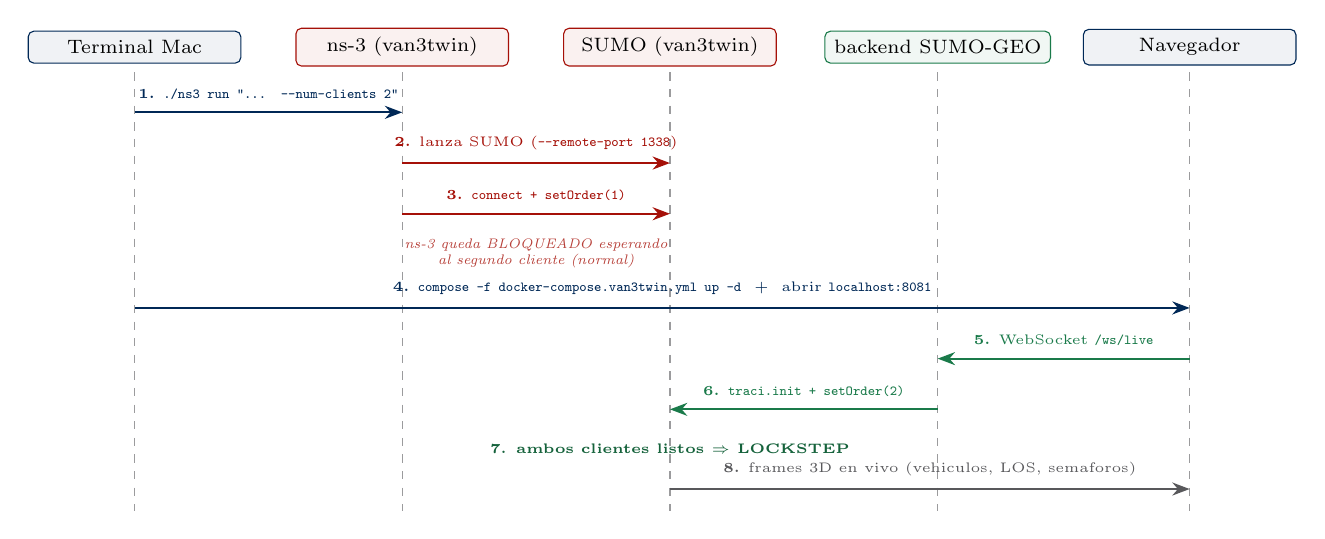
\begin{tikzpicture}[font=\scriptsize, yscale=0.92]
  % lifelines
  \foreach \x/\n/\c in {0/{Terminal Mac}/azul, 3.4/{ns-3 (van3twin)}/rojo,
                        6.8/{SUMO (van3twin)}/rojo, 10.2/{backend SUMO-GEO}/verde,
                        13.4/{Navegador}/azul}{
    \node[draw=\c, fill=\c!6, rounded corners=2pt, minimum width=2.7cm] (h\x) at (\x,0) {\n};
    \draw[gris!60, dashed] (\x,-0.35) -- (\x,-6.4);
  }
  \newcommand{\msg}[5]{\draw[-{Stealth[length=2.2mm]}, thick, #4] (#1,#3) -- (#2,#3)
        node[midway, above=1pt, align=center, font=\tiny] {#5};}
  \msg{0}{3.4}{-0.9}{azul}{\textbf{1.} \texttt{./ns3 run "... --num-clients 2"}}
  \msg{3.4}{6.8}{-1.6}{rojo}{\textbf{2.} lanza SUMO (\texttt{--remote-port 1338})}
  \msg{3.4}{6.8}{-2.3}{rojo}{\textbf{3.} \texttt{connect + setOrder(1)}}
  \node[rojo!80, font=\tiny\itshape, align=center] at (5.1,-2.85)
        {ns-3 queda BLOQUEADO esperando\\al segundo cliente (normal)};
  \msg{0}{13.4}{-3.6}{azul}{\textbf{4.} \texttt{compose -f docker-compose.van3twin.yml up -d} ~+~ abrir \texttt{localhost:8081}}
  \msg{13.4}{10.2}{-4.3}{verde}{\textbf{5.} WebSocket \texttt{/ws/live}}
  \msg{10.2}{6.8}{-5.0}{verde}{\textbf{6.} \texttt{traci.init + setOrder(2)}}
  \node[verde!80!black, font=\tiny\bfseries] at (6.8,-5.55) {7. ambos clientes listos $\Rightarrow$ LOCKSTEP};
  \msg{6.8}{13.4}{-6.1}{gris}{\textbf{8.} frames 3D en vivo (vehiculos, LOS, semaforos)};
\end{tikzpicture}
\caption{Secuencia de arranque. El paso 3 se bloquea hasta el paso 6 (hecho validado \#2):
por eso ns-3 debe lanzarse \emph{antes} de abrir el visor.}
\label{fig:secuencia}
\end{figure}

\begin{enmac}[ --- 1) levantar van3twin]
\begin{lstlisting}[language=bash]
cd ~/van3twin-docker && docker compose up -d
\end{lstlisting}
\end{enmac}

\begin{encontenedor}[ --- 2) lanzar la simulación EVA con 2 clientes TraCI]
\begin{lstlisting}[language=bash]
docker compose exec van3twin bash     # (desde el Mac)

# dentro del contenedor:
./ns3 run "v2v-emergencyVehicleAlert-80211p --sumo-gui=false --met-sup=true \
  --ns3::TraciClient::SumoAdditionalCmdOptions='--num-clients 2'"
# -> ns-3 lanza SUMO y queda ESPERANDO al segundo cliente
\end{lstlisting}
La sintaxis \texttt{--ns3::TraciClient::SumoAdditionalCmdOptions=...} fija el atributo
desde la línea de comandos \emph{sin tocar el código del ejemplo}: el ejemplo EVA no
asigna ese atributo y \texttt{traci-client.cc:240} concatena su valor al comando de SUMO.
Puedes añadir tus flags habituales (\texttt{--csv-log}, \texttt{--penetrationRate}, \ldots).
\end{encontenedor}

\begin{enmac}[ --- 3) levantar SUMO-GEO y abrir el visor]
\begin{lstlisting}[language=bash]
cd /ruta/a/SUMO_GEO
docker compose -f docker-compose.van3twin.yml up -d --build

open http://localhost:8081     # al abrirse el WebSocket arranca el lockstep
\end{lstlisting}
\end{enmac}

% ============================================================================
\section{Paso 6 — Verificación}
% ============================================================================

\begin{enmac}[ --- comprobaciones]
\begin{lstlisting}[language=bash]
# backend sin errores de conexion TraCI ni de version:
docker compose -f docker-compose.van3twin.yml logs backend

# API viva:
curl http://localhost:8000/api/health
\end{lstlisting}
\end{enmac}

En el visor (\texttt{localhost:8081}) debe verse: los 7--8 vehículos del escenario EVA
sobre el mapa real del ejemplo (zona de Turín) como cajas 3D orientadas, el color LOS por
calle, el inspector de clic derecho (velocidad, \emph{edge}, CO$_2$, espera\ldots) y el
panel de históricos. Al avanzar ns-3, los vehículos se mueven en el navegador
\emph{en el mismo instante simulado}.

\begin{center}
\begin{tabular}{@{}lll@{}}
\toprule
\textbf{Puerto (Mac)} & \textbf{Servicio} & \textbf{Stack} \\
\midrule
8081 & Frontend SUMO-GEO (visor 3D)            & SUMO-GEO \\
8000 & Backend FastAPI (REST + WS)             & SUMO-GEO \\
8080 & vehicle-visualizer de VaN3Twin          & van3twin \\
5901 & VNC (GUI del contenedor)                & van3twin \\
8090 & GEO SUMO WEB (modo vivo, práctica)      & van3twin \\
---  & TraCI 1338: \emph{no publicado} (solo red interna Docker) & ambos \\
\bottomrule
\end{tabular}
\end{center}

% ============================================================================
\section{Tarea del taller — 7 vehículos + vehículo de emergencia}
% ============================================================================

Objetivo: preparar un escenario propio y observarlo en el visor 3D. Se parte del
escenario de \textbf{7 vehículos} (\texttt{map\_7.sumo.cfg}, que habilita
\texttt{cars\_7.rou.xml}) en
\texttt{src/automotive/examples/sumo\_files\_v2v\_map/}.

\begin{notabox}[: editar con Visual Studio Code desde el Mac]
Gracias al bind mount, los archivos de SUMO son archivos normales del Mac.
Se recomienda abrirlos con VS Code --- no hace falta editar dentro del contenedor
ni recompilar nada: SUMO los lee al arrancar cada simulación.
\begin{lstlisting}[language=bash]
code ~/van3twin-docker/VaN3Twin/ns-3-dev/src/automotive/examples/sumo_files_v2v_map
# (o VS Code -> File -> Open Folder... si el comando 'code' no esta en el PATH)
\end{lstlisting}
\end{notabox}

\begin{tallerbox}
\begin{enumerate}[leftmargin=1.6em, itemsep=3pt]
  \item \textbf{Habilitar el escenario de 7 vehículos.} No hay que editar ningún
        \texttt{.sumocfg}: el ejemplo acepta \texttt{--sumo-config} y
        \texttt{map\_7.sumo.cfg} ya apunta a \texttt{cars\_7.rou.xml}
        (7 vehículos tipo \texttt{Car1}, 6{,}94~m/s).
  \item \textbf{Añadir un vehículo de emergencia} en \texttt{cars\_7.rou.xml}.
        Este fichero \emph{no} define ningún tipo \texttt{emergency}: copiar el
        vType \texttt{Car0} del \texttt{cars.rou.xml} original y añadir la
        ambulancia como octavo vehículo:
\begin{lstlisting}
<vType accel="4" decel="7.5" emergencyDecel="10" minGap="1.0"
       id="Car0" vClass="emergency" maxSpeed="20.83"/>
...
<vehicle id="veh8" type="Car0" depart="5" route="0">
</vehicle>
\end{lstlisting}
        La clave es \texttt{vClass="emergency"}: la app la detecta con
        \texttt{vehicle.getVehicleClass()} (\texttt{emergencyVehicleAlert.cc:166})
        y sus CAMs llevan \texttt{stationType = specialVehicle(10)}. Que salga
        \emph{tarde} (\texttt{depart="5"}) y \emph{rápida} (20{,}83 vs.\
        6{,}94~m/s) garantiza que alcance al pelotón.
  \item \textbf{Misma ruta para todos.} Verificar/modificar que TODOS los
        \texttt{<vehicle>} llevan \texttt{route="0"} --- la misma que la
        ambulancia. La reacción EVA exige distancia bajo umbral \emph{y} rumbo
        similar: solo se dispara si comparten trayecto.
  \item \textbf{Ejecutar con el visor 3D} (Pasos 5.2--5.3 de esta guía):
\begin{lstlisting}[language=bash]
./ns3 run "v2v-emergencyVehicleAlert-80211p --sumo-gui=false --met-sup=true \
  --sumo-config='src/automotive/examples/sumo_files_v2v_map/map_7.sumo.cfg' \
  --ns3::TraciClient::SumoAdditionalCmdOptions='--num-clients 2'"
\end{lstlisting}
  \item \textbf{Entregable:} captura del visor (\texttt{localhost:8081}) con la
        ambulancia alcanzando al pelotón + 3--5 líneas: ¿qué hacen los
        \texttt{Car1} al recibir sus CAMs (velocidad/carril con el inspector de
        clic derecho) y a qué distancia reaccionan?
\end{enumerate}
\end{tallerbox}

% ============================================================================
\section{Límites y notas de operación}
% ============================================================================

\begin{itemize}[leftmargin=1.4em, itemsep=2pt]
  \item \textbf{Un visor por corrida.} \texttt{--num-clients} fija el número de clientes al
        arranque de SUMO. No usar el selector Bajo/Medio/Alto en este modo (reconectaría a
        un SUMO ``gestionado'' que aquí no existe); si se recarga la página a mitad de
        corrida, puede hacer falta relanzar el Paso~5.2.
  \item \textbf{Fin de la simulación.} VaN3Twin arranca SUMO con \texttt{--quit-on-end}:
        al terminar, SUMO se cierra y el visor pierde la conexión. Es lo esperado.
  \item \textbf{Qué muestra cada visor.} SUMO-GEO $=$ \emph{verdad terreno} de SUMO en 3D
        (todos los vehículos); GEO SUMO WEB 2D/3D (carpeta de la práctica) $=$
        \emph{percepción por radio} (CAMs por receptor); \texttt{vehicle-visualizer}
        (\texttt{:8080}) $=$ verdad terreno 2D nativa de VaN3Twin. Son complementarios.
  \item \textbf{Versiones.} Si se actualiza el SUMO del contenedor van3twin, actualizar
        los pines \texttt{traci}/\texttt{sumolib} del Paso~3 para que coincidan.
  \item \textbf{Rendimiento.} El ritmo lo marca ns-3; el visor añade una carga de lectura
        ligera (suscripciones TraCI, hecho validado \#1). Con \texttt{APP\_MAX\_FPS=10} y
        \texttt{APP\_STEP\_LENGTH=1.0} el visor concede hasta 10~s simulados por segundo
        real: nunca es el cuello de botella.
\end{itemize}

\vspace{6pt}
\hrule
\vspace{4pt}
{\small\color{gris} Repos: \url{https://github.com/Pbarbecho/SUMO_GEO} \,·\,
\url{https://github.com/DriveX-devs/VaN3Twin}. Guía complementaria:
\texttt{GUIA\_INTEGRACION\_SUMO\_GEO.md} y manual
\texttt{VaN3Twin\_Docker\_macOS.pdf} en \texttt{van3twin-docker/}.}

\end{document}
